\documentclass[UTF8]{ctexart}

\usepackage{amsmath}
\usepackage{multicol}
\setlength{\parindent}{2em}
\addtolength{\topmargin}{-54pt}
\setlength{\oddsidemargin}{0.63cm}  % 3.17cm - 1 inch
\setlength{\evensidemargin}{\oddsidemargin}
\setlength{\textwidth}{14.66cm}
\setlength{\textheight}{24.00cm}    % 24.62
\usepackage{graphicx}
\usepackage{float}
\usepackage{multirow}
\usepackage{subfigure}
\usepackage{multirow}
\begin{document}

%标题
\begin{center}
\Huge\textbf{铷原子的光泵磁共振实验}
\renewcommand{\baselinestretch}{5.0}
\end{center}
\begin{center}
\small
\begin{tabular}{llll}
\textbf{姓名}&李励玮     &\textbf{学号}  &201711140236\\
\textbf{指导老师}&王海燕 &\textbf{实验日期}& 2019.12.13\\
\end{tabular}
\end{center}

%摘要
\small
\noindent\textbf{摘要}:电子吸收圆偏振光后能发生光抽运现象,可以用扫场的方法来观察到该现象;在另加线偏振射频场的情况下,塞曼子能级间发生磁共振,也可以用扫场的方法观察;根据磁共振时测得的水平场可以计算得原子的$g_F$因子和地磁场大小。
\newline\textbf{关键字:光抽运、磁共振、$g_F$因子、地磁场}

\begin{multicols}{2}
%引言
\section{引言}
在磁场中, Zeeman分裂导致的磁能级间距通常比较小,因此,产生磁共振现象所需的能量通常位于射频或微波波段,能量要比光频段的能量小得多,普通的光谱仪器无法分辨,所以对于磁共振信号很微弱的样品(比如气体样品)很难探测。

光泵,也称光抽运,是借助于光辐射获得原子基态超精细结构能级或 Zeeman子能级间粒子数的非热平衡分布的实验方法。

在光泵磁共振技术中,一方面光抽运改变了磁能级上的粒子数分布,使更多的粒子参与磁共振,另一方面采取光探测的方法而不直接测量射频量子,从而克服了磁共振信号弱的缺点,把探测灵敏度提高了七、八个数量级。

如今,光泵磁共振已广泛应用于基础物理研究,比如原子的磁矩、能级结构和g因子测量以及原子频标、激光和弱磁场测量。

\section{实验目的}
理解光抽运的物理过程、了解光泵磁共振的原理,研究铷Rb原子的光泵磁共振现象,并测量Rb的朗德g因子、地磁场的水平、垂直分量。

\section{实验原理}
\subsection{Rb原子基态及最低激发态能级}
Rb是碱金属原子,其最外层有一个价电子,位于5s能级上,故电子轨道量子数$L=0$,自旋量子数$S=\frac{1}{2}$,L-S耦合得总角动量。因此,基态为$5^2S_{\frac{1}{2}}$。

第一激发态$L=1$,$S=\frac{1}{2}$,故有双重态$5^2P_{\frac{1}{2}}$、$5^2P_{\frac{3}{2}}$。

核自旋量子数$I=0$时,总角动量$P_J$与总磁矩$\mu_J$关系为:
\begin{equation}
\begin{array}{l}{\mu_{J}=-g_{J} \frac{e}{2 m_{e}} P_{J}} \\ {g_{J}=1+\frac{J(J+1)-L(L+1)+S(S+1)}{2 J(J+1)}}\end{array}
\end{equation}
$I=0$,总角动量$P_F$与总磁矩$\mu_F$关系为:
\begin{equation}
\begin{aligned} \mu_{F} &=-g_{F} \frac{e}{2 m_{e}} P_{F} \\ g_{F} &=g_{J} \frac{F(F+1)+J(J+1)-I(I+1)}{2 F(F+1)} \end{aligned}
\end{equation}
$^{87} \mathrm{Rb}$的$I=\frac{3}{2}$,故基态$F=2,1$;$^{85} \mathrm{Rb}$的$I=\frac{5}{2}$,故基态$F=3,2$。

在磁场中原子的超精细结构能级产生Zeeman分裂,当磁场较弱时为反常 Zeeman分裂,磁量子数$m_F=F,F-1,...,-F$,产生$2F+1$个能级间距基本相等的 Zeeman子能级。

弱磁场条件下Rb原子能量本征值
\begin{equation}
E=E_{0}+\frac{a h}{2}[F(F+1)-J(J+1)-I(I+1)]+g_{F} m_{F} \mu_{B} B_{0}
\end{equation}
故相邻Zeeman子能级间能量
\begin{equation}
\Delta E_{m_{F}}=g_{F} \mu_{B} B_{0}
\end{equation}

\subsection{圆偏振光对Rb原子的激发与光抽运效应}
电子跃迁时,需满足原子和光子的总能量和总角动量要守恒。能量守恒要求光子的能量hv与跃迁能级间的能量变化相等;角动量是矢量,在考虑角动量守恒时还需要考虑光的偏振状态。
左旋圆偏振光和右旋圆偏振光分别用$\sigma^-$和$\sigma^+$表示,角动量分别为$\hbar$和$-\hbar$,其方向分别光的传播方向相同和相反指向光的传播方向。所以,当电子吸收左旋圆偏振光后,量子力学给出的跃迁选择定则为:
\begin{equation}
\begin{array}{l}{\Delta L=\pm 1} \\ {\Delta F=0, \pm 1} \\ {\Delta m_{F}=+1}\end{array}
\end{equation}
\noindent\textbf{光抽运效应}:Rb的基态$5^2S_{\frac{1}{2}}$和第一激发态$5^2P_{\frac{1}{2}}$的磁量子数的最大值都是$+2$,若用Rb光谱的$D_1$线的$\sigma^+$光激发Rb原子,$5^2S_{\frac{1}{2}}$的$m_F=+2$子能级上的粒子不能被激发至$5^2P_{\frac{1}{2}}$态;当原子从$5^2P_{\frac{1}{2}}$经历自发辐射和无辐射跃迁回到$5^2S_{\frac{1}{2}}$时,粒子返回基态各个子能级的几率大致相等,经过若干循环之后,基态$m_F=+2$子能级上的粒子数积累,即大量粒子被“抽运”到$m_F=+2$的子能级上。

同理,$\sigma^+$光将粒子抽运到基态子能级$m_F=-2$上。

各子能级上粒子数的这种不均匀分布叫做“偏极化”。光抽运的目的就是要实现粒子分布的偏极化。

\subsection{弛豫过程}
光抽运使得个别子能级上的粒子数大大的增加,使系统处于非热平衡状态。系统由非热平衡分布状态趋向于热平衡分布状态的过程称为弛豫过程。弛豫的微观过程在Rb原子系统中主要有以下几种:
\newline\textbf{(1)Rb原子与容器壁的碰撞。}这种碰撞会导致子能级之间的跃迁,使原子恢复到热平衡分布,失去光抽运所造成的偏极化。
\newline\textbf{(2)Rb原子之间的碰撞。}这种碰撞导致自旋一自旋交换弛豫,使粒子的磁矩发生改变从而失去偏极化。当外场为零时,Zeeman子能级简并,是通过这种过程使原子回到热平衡分布。
\newline\textbf{(3)Rb原子与缓冲气体之间的碰撞。}
\newline\textbf{a.}通常选择分子磁性很小的气体作为缓冲气体,这样,缓冲气体与原子的碰撞对的磁能态扰动极小,基本对原子的偏极化没有影响。原子与器壁碰撞是失去偏极化的主要原因,充入缓冲气体后,将大大减少Rb原子与器壁碰撞的机会,从而保持了原子高度的偏极化。缓冲气体主要作用是使基态由非热平衡分布恢复到热平衡分布的弛豫时间增加。
\newline\textbf{b.}处于$5^2P_{\frac{1}{2}}$态的原子需与缓冲气体分子碰撞多次才有可能发生能量转移,而且主要是以无辐射跃迁的形式交换能量,所以返回到基态八个Zeeman子能级的几率均等,因此缓冲气体分子还有将粒子更快地抽运到$m_F=+2$子能级的作用。

温度升高,Rb蒸汽原子密度升高,Rb原子与器壁及Rb原子之间的碰撞都增加,使原子的偏极化减小。而当温度过低时,原子数太少,信号幅度也很小。Rb原子蒸汽的最佳温度范围一般应控制在40℃-60℃之间。

\subsection{Zeeman子能级之间的磁共振}
在垂直于恒定磁场$\vec{B}_{0}$的方向上加一圆频率$\omega_1$(满足$\hbar \omega_{1}=\Delta E_{m F}=g_{F} \mu_{B} B_{0}$)的线偏振射频场$\vec{B}_{1}$, Zeeman子能级之间将产生磁共振,即被抽运到基态$m_F=+2$子能级上的大量粒子在$\vec{B}_{1}$的作用,由$m_F=+2$跃迁到$m_F=+1$。因此又发生光抽运,对$D_1$光吸收增加,最后感应跃迁与光抽运将达到一个新的动态平衡。
\subsection{光探测}
射入样品泡的D线的$\sigma^+$光一方面起光抽运的作用;另一方面,发生磁共振时,样品对
D1线的$\sigma^+$光吸收强度发生改变,因此测量其透过样品后的光强变化即可得到相关的磁共振信号,从而实现了对磁共振的光探测。

\section{实验装置}
\begin{figure}[H]
\centering
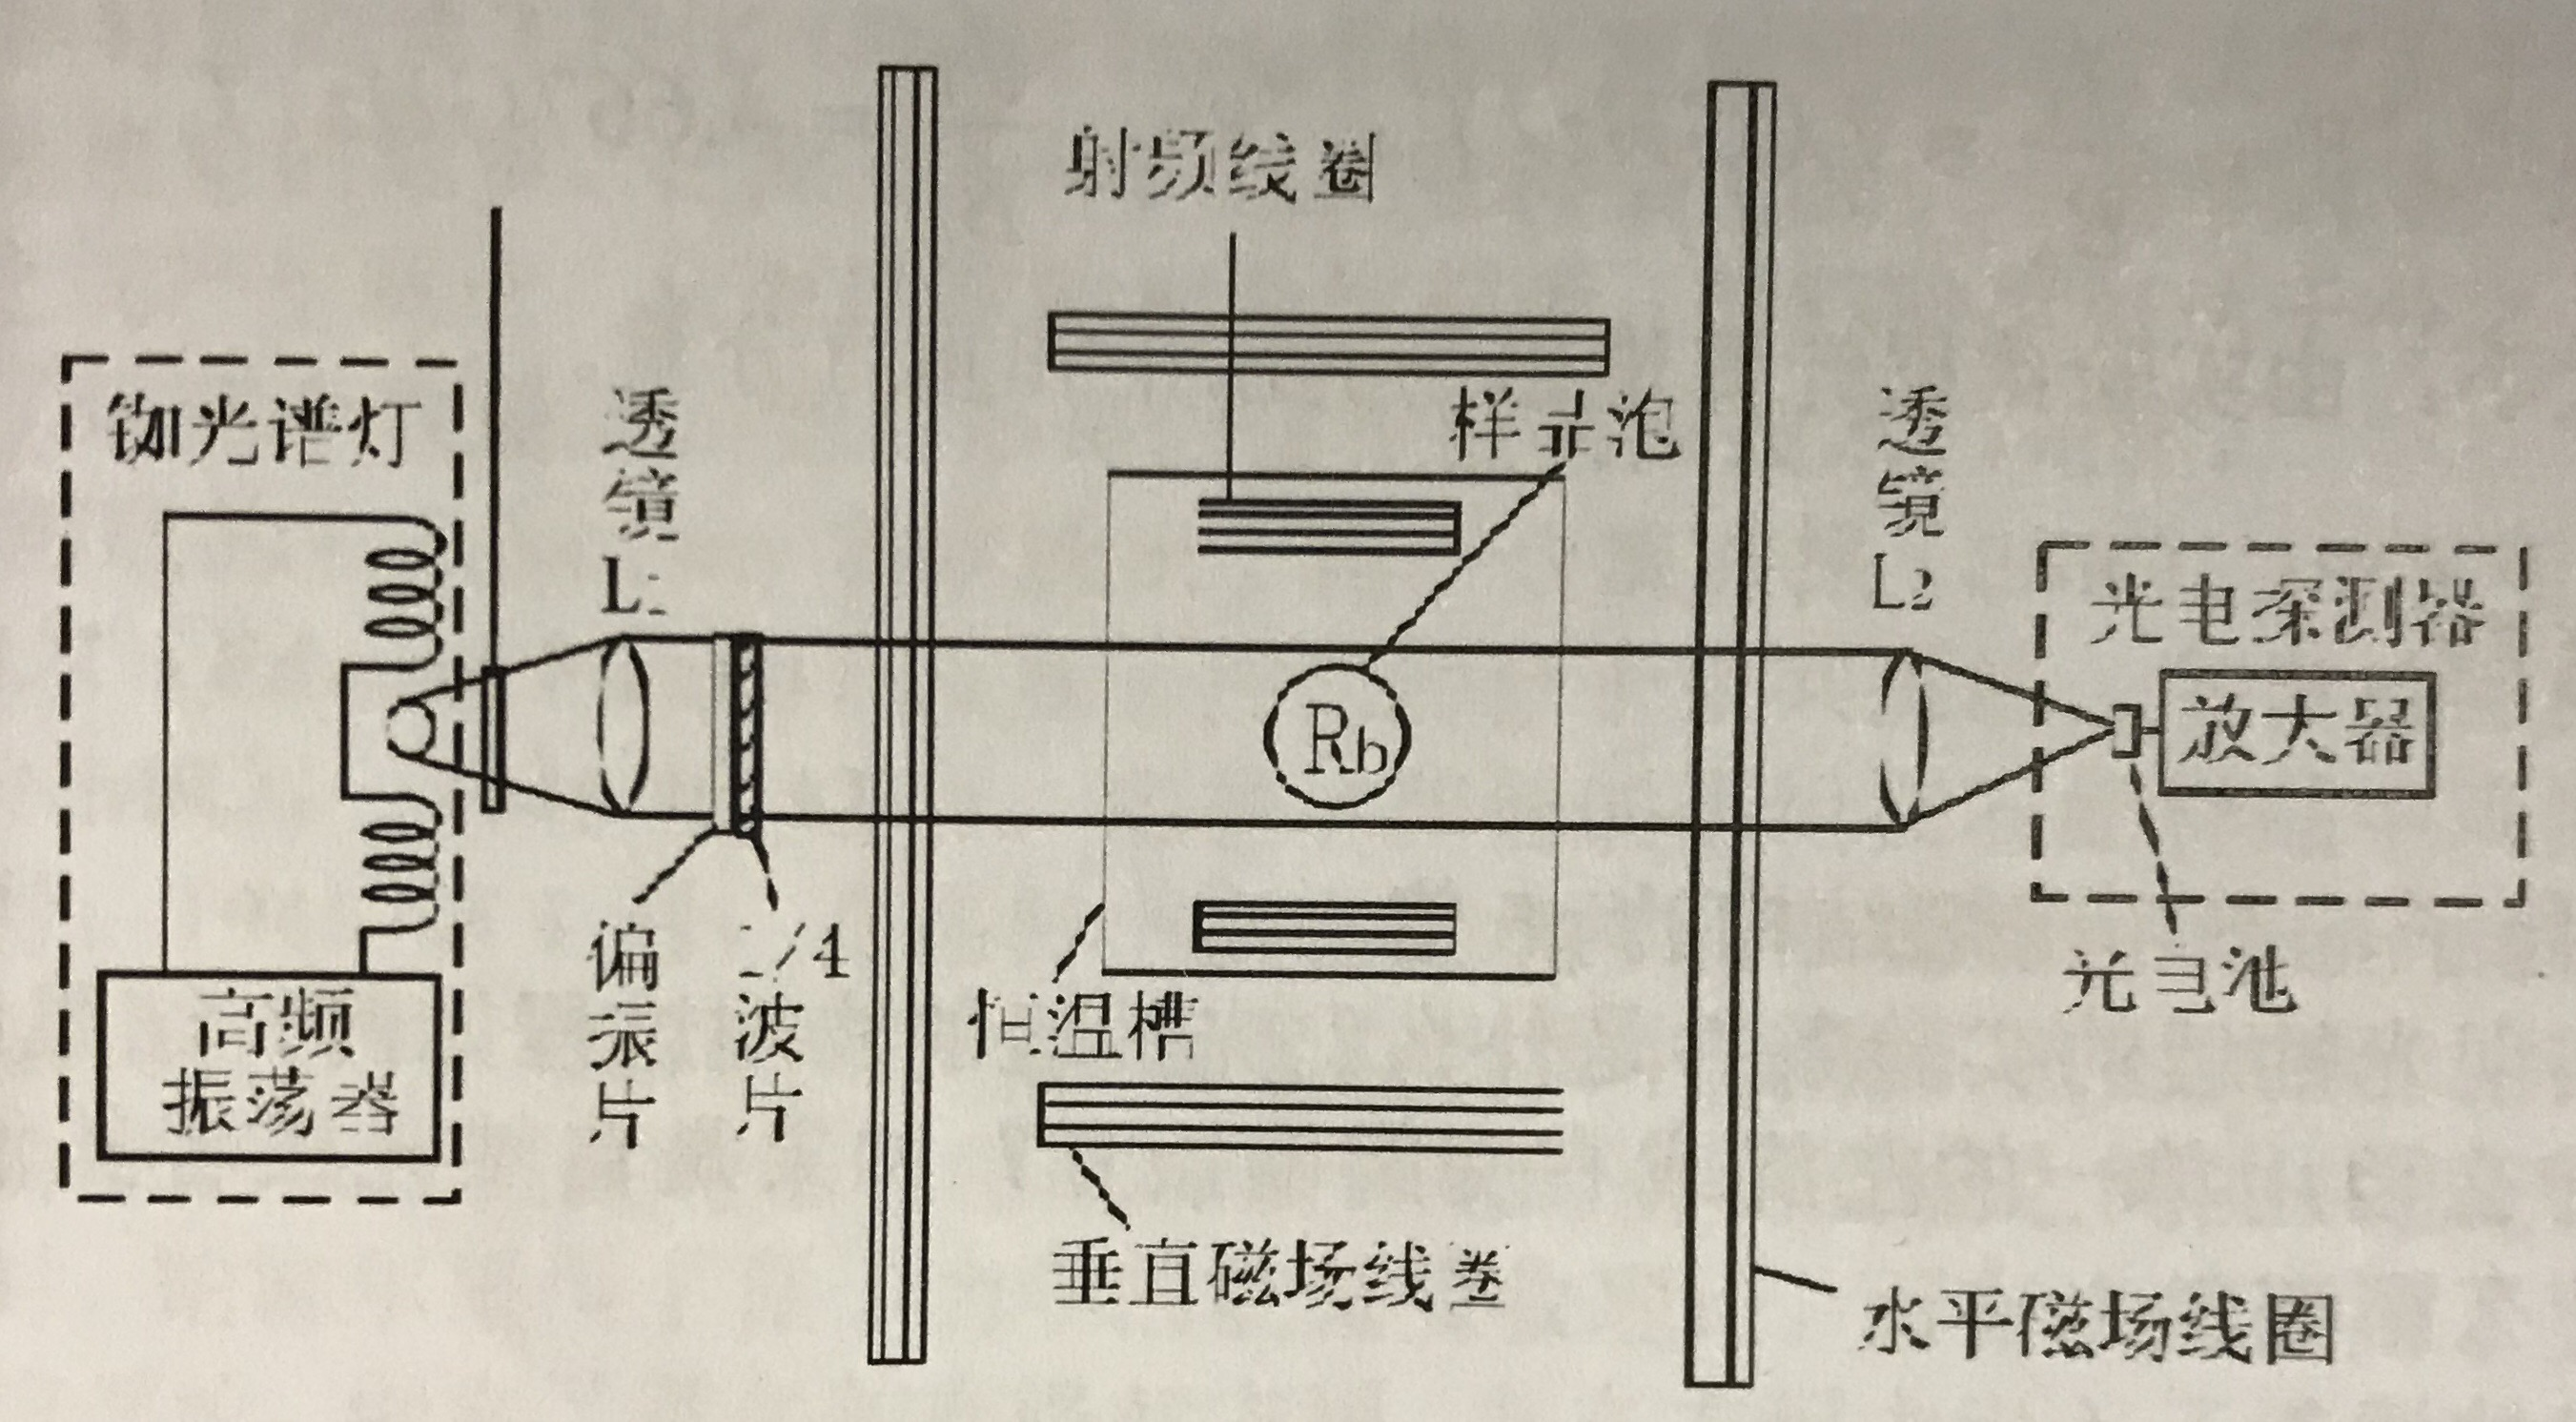
\includegraphics[width=7cm]{lightroot}
\caption{\small{实验装置}}
\end{figure}
本实验采用的Rb原子光泵磁共振实验装置如图所示。\textbf{光源}采用高频无极放电Rb灯,其优点是稳定性好,噪音小,光强大。由于D2线的存在不利于D1线的光抽运,故用透过率大于60%,带宽小于15nm的\textbf{干涉滤光片}就能很好地滤去D2线。用高碘硫酸奎宁\textbf{偏振片}和40pm左右的云母\textbf{$1/4$波片}可产生左旋圆偏振光$\sigma^+$。\textbf{透镜$L_1$}可将光源发出的光变为平行光。\textbf{透镜$L_2$}将透过样品泡的平行光会聚到光电接受器上。

产生\textbf{水平磁场的亥姆霍兹线圈}的轴线与地磁场水平分量方向一致(即应指向南北方向),其大小$B_0$在$0~2GS$连续可调。水平方向\textbf{扫场信号}的调节范围为几十毫GS至1GS左右,扫场信号的输出方式有方波和三角波两种,并与示波器的扫描同步。产生\textbf{垂直磁场的亥姆霍兹线圈}用以抵消地磁场的垂直分量,以获得最佳的共振信号。\textbf{射频线圈}放在样品泡两侧并使$\vec{B}_{1}$垂直于$\vec{B}_{0}$,射频信号由信号发生器产生,其频率由几百KHz到几MHz,功率由几mW到1W或更大些。

\textbf{样品泡}是一个充有适量天然Rb、直径约5cm的玻璃泡,泡内还充有约10Torr的氮、氩等缓冲气体。样品泡放在恒温室中,温度可控制在30℃-70℃之间,且温度的波动小于$\pm1℃$。\textbf{光检测器}由光电接收器及放大电路组成。光电接收元件可采用光电管或光电池。光电管响应速度快;光电池较慢,但光电池受光面积大、内阻低。本实验采用光电池。\textbf{放大电路}最好用直流耦合电路,波形畸变小。当不测量光抽运时间及弛豫时间时,用交流耦合电路也可以。

\section{实验内容}
\noindent\textbf{1.加热样品泡和Rb灯。}

通常样品泡的温度应稳定在$40-60℃$之间,而Rb灯的温度控制在$90℃$左右。待“灯温”、“池温”的指示灯亮后,就可以开始做实验。
\newline\textbf{2.消除地磁场垂直分量对信号的影响、观察光抽运信号。}

将扫场线圈的输出方式设为方波,调节其振幅使磁场为$0.5-1GS$。加上外磁场的瞬间,基态各Zeeman子能级上的粒子数仍接近热平衡分布,即可认为各子能级上的粒子数大致相等,因此,这一瞬间有总粒子数的7/8可吸收D1的光,对光的吸收最强。随着粒子逐渐被抽运到$m_F=+2$子能级上,能够吸收光的粒子数逐渐减少,因而透过样品的光强逐渐增加。当$m_F=+2$子能级上的粒子数达到饱和时,透过样品的光强达到最大。方波扫过零并反向时, Zeeman子能级随之发生简并及再分裂,能级简并时,Rb原子因碰撞导致自旋方向混乱而失去偏极化。重新分裂后,各Zeeman子能级的粒子数又近似相等,对D1光的吸收又达最大值。这就是光抽运信号。

地磁场对光抽运信号有很大影响,特别是地磁场的垂直分量。因此安装了一对垂直方向的亥姆霍兹线圈以抵消其影响。当垂直方向总磁场为零时,地磁场的垂直分量被抵消,光抽运的信号最大。
\newline\textbf{3.观察磁共振信号。}

在本实验中采用扫场法测量磁共振信号,即保持射频场的频率不变,通过改变稳恒磁场的大小得到共振信号。首先给样品泡加上射频场B,扫场信号选择锯齿波输出,改变水平磁场的大小,测量$^{87} \mathrm{Rb}$及$^{85} \mathrm{Rb}$发生共振时磁场的大小。由实验数据计算$^{85} \mathrm{Rb}$及$^{87} \mathrm{Rb}$的$g_F$值、地磁场的水平分量$B_{\|}$和垂直分量$B_{\perp}$,并与理论值进行比较。

\end{multicols}

\section{实验结果分析与讨论}
\noindent\textbf{1.观察光抽运信号}
\newline\textbf{(1)水平场为正,扫场为负}
\begin{figure}[H]
\centering
\subfigure[扫场上沿恰为总磁场为0]{
\label{fig:subfig:a}
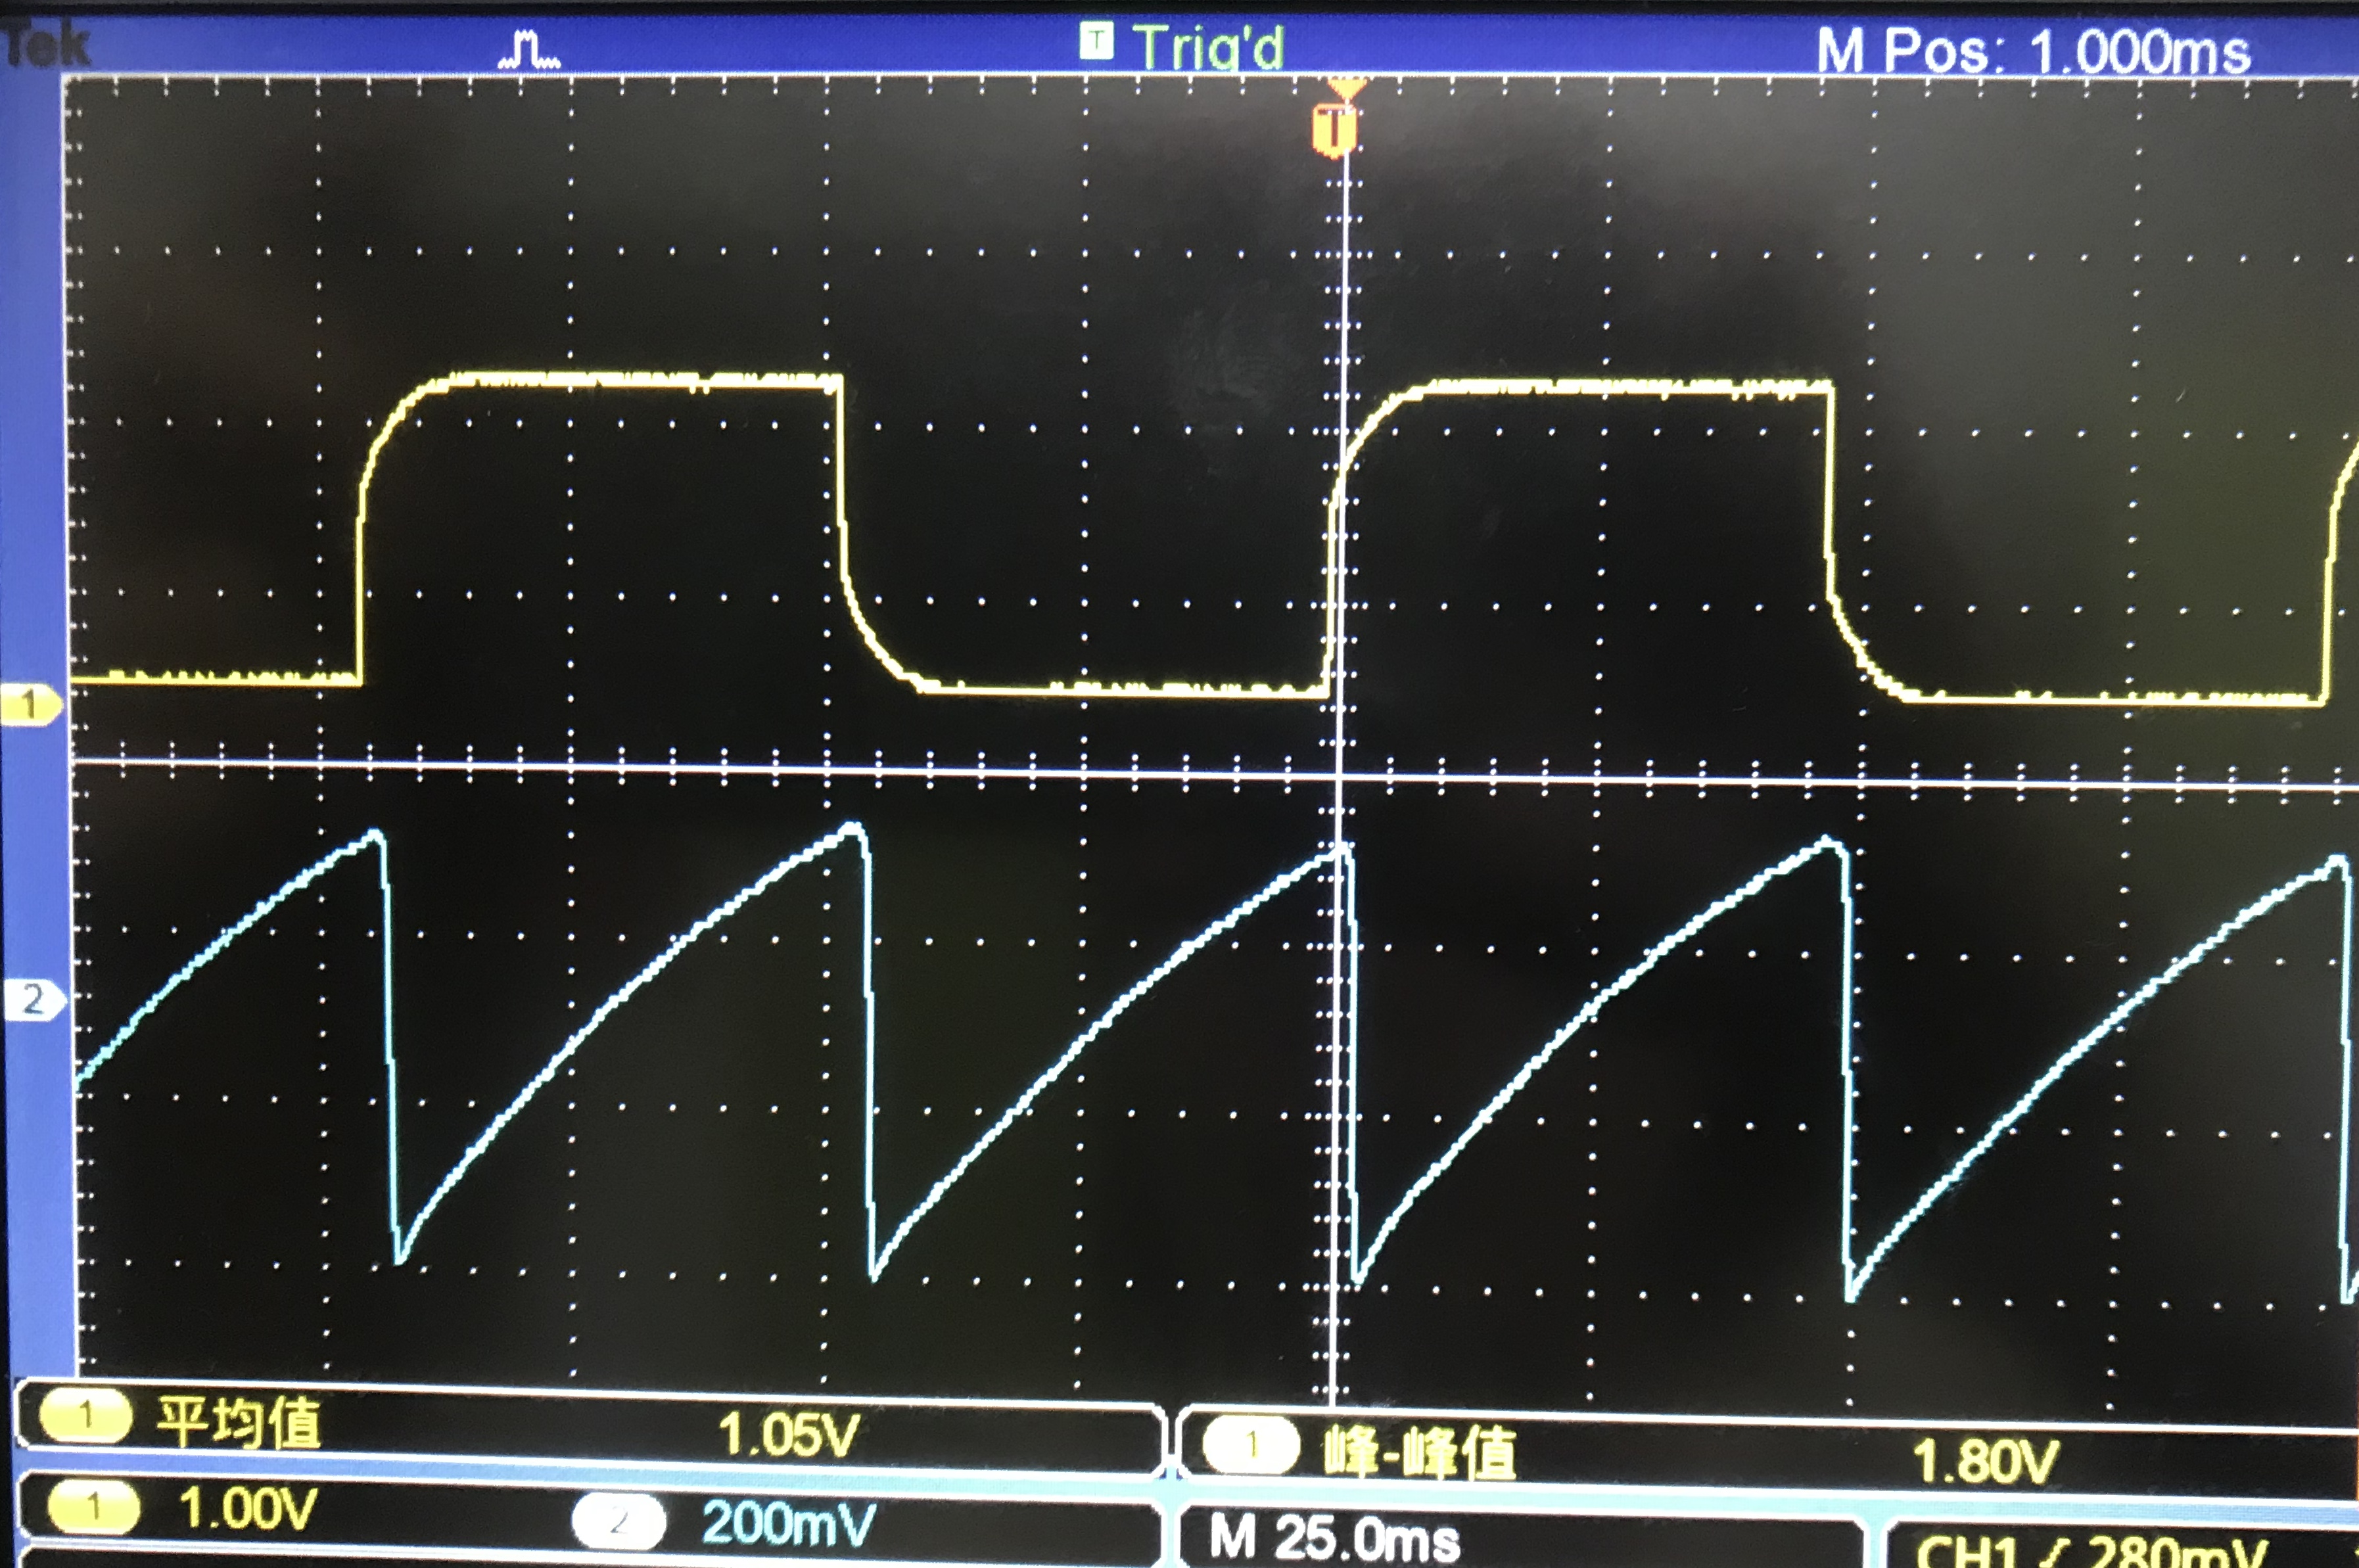
\includegraphics[width=6cm]{12}
}
\subfigure[扫场中点恰为总磁场为0]{
\label{fig:subfig:b}
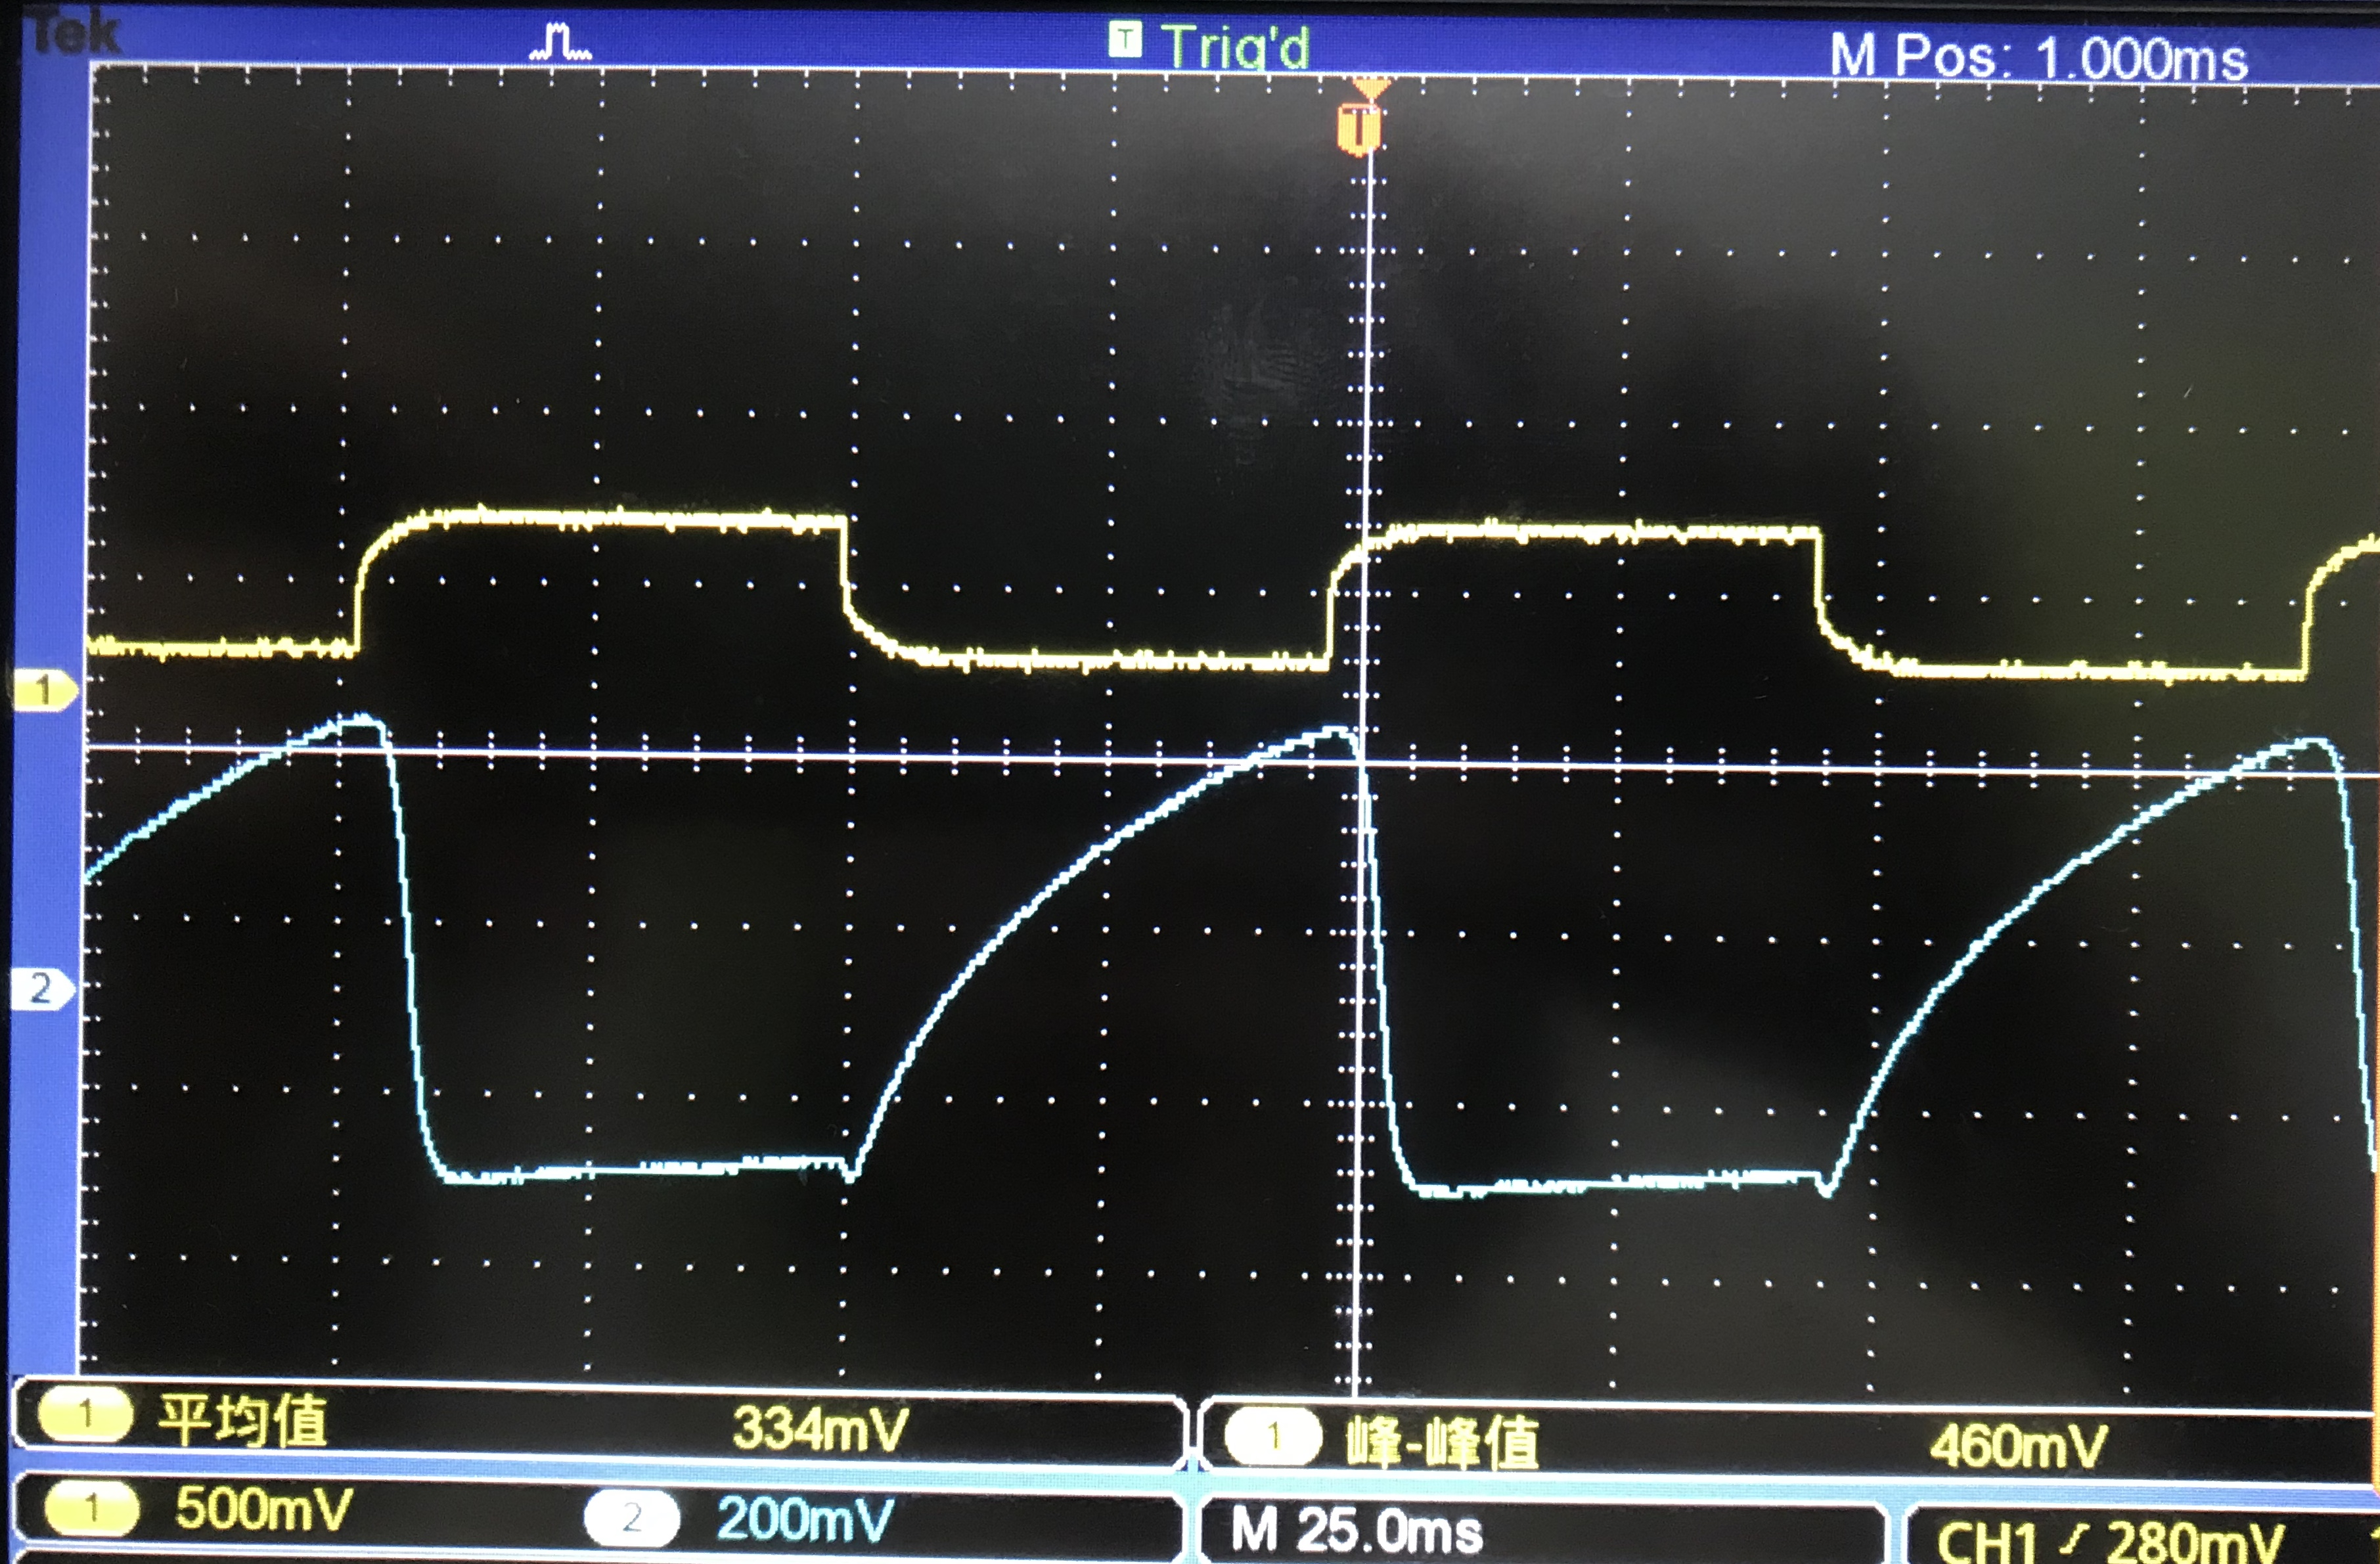
\includegraphics[width=6cm]{11}
}
\end{figure}
\noindent\textbf{(2)水平场为负,扫场为负}
\begin{figure}[H]
\centering
\subfigure[扫场下沿恰为总磁场为0]{
\label{fig:subfig:a}
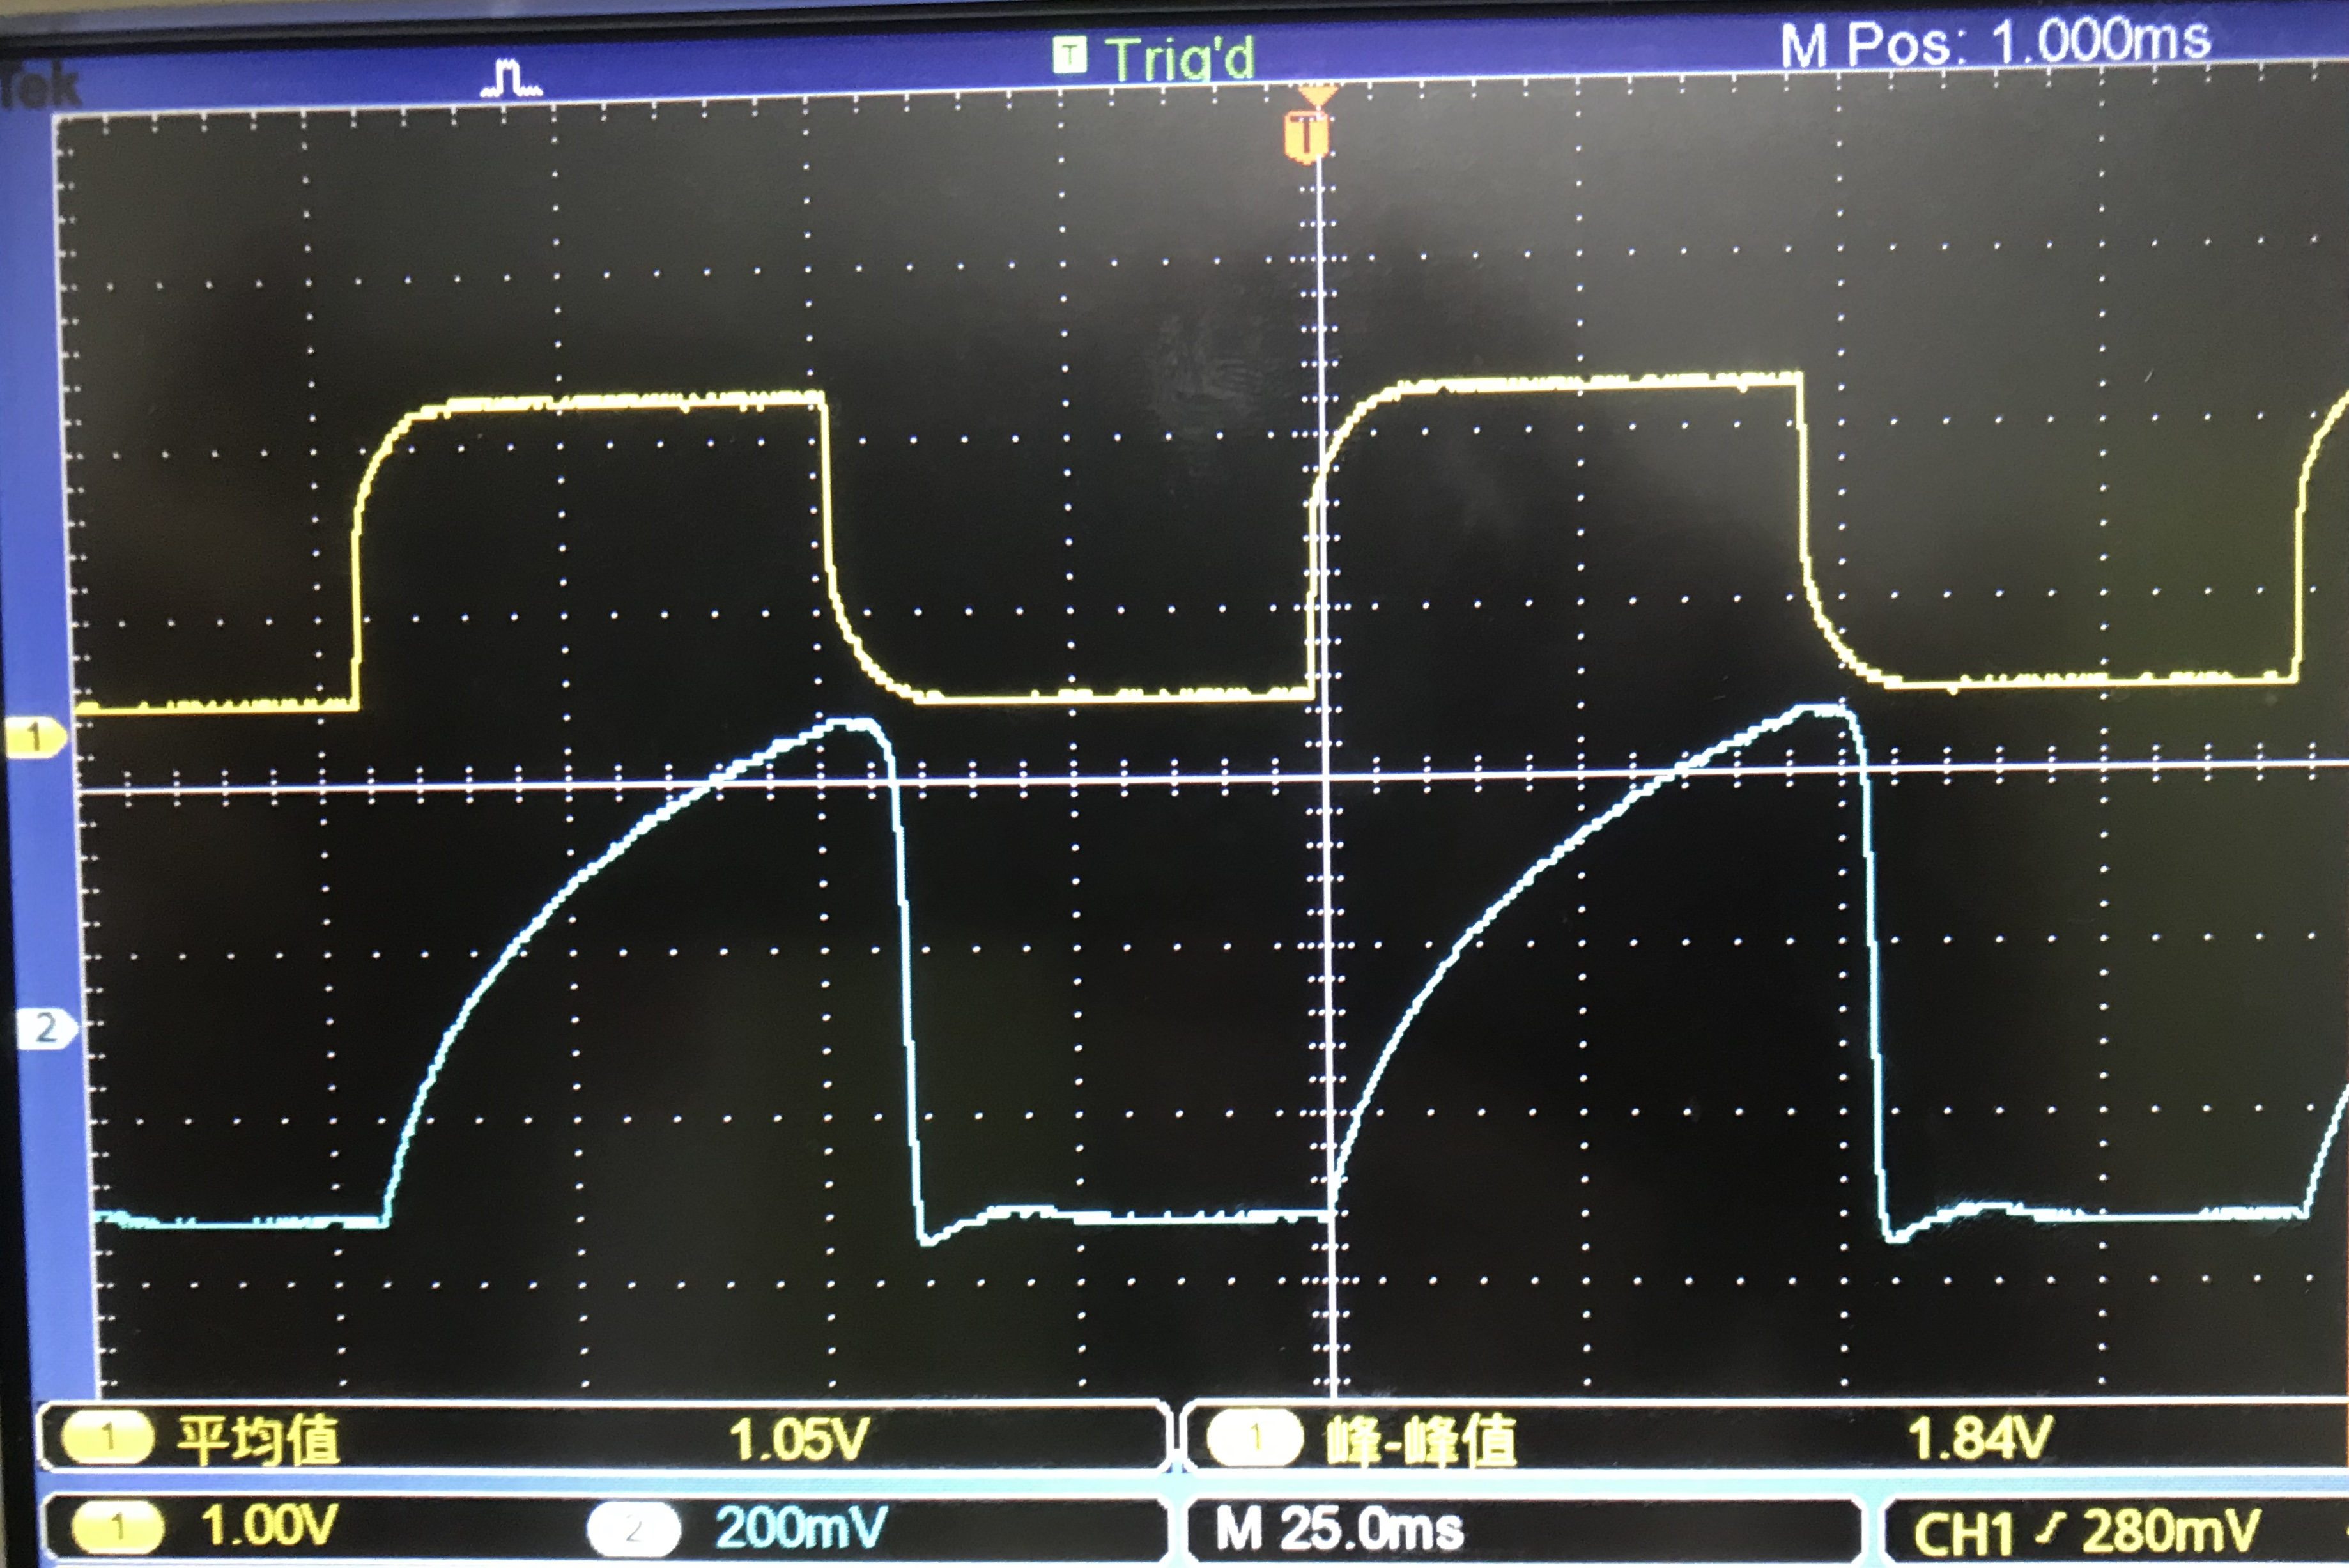
\includegraphics[width=4.3cm]{21}
}
\subfigure[扫场中点恰为总磁场为0]{
\label{fig:subfig:b}
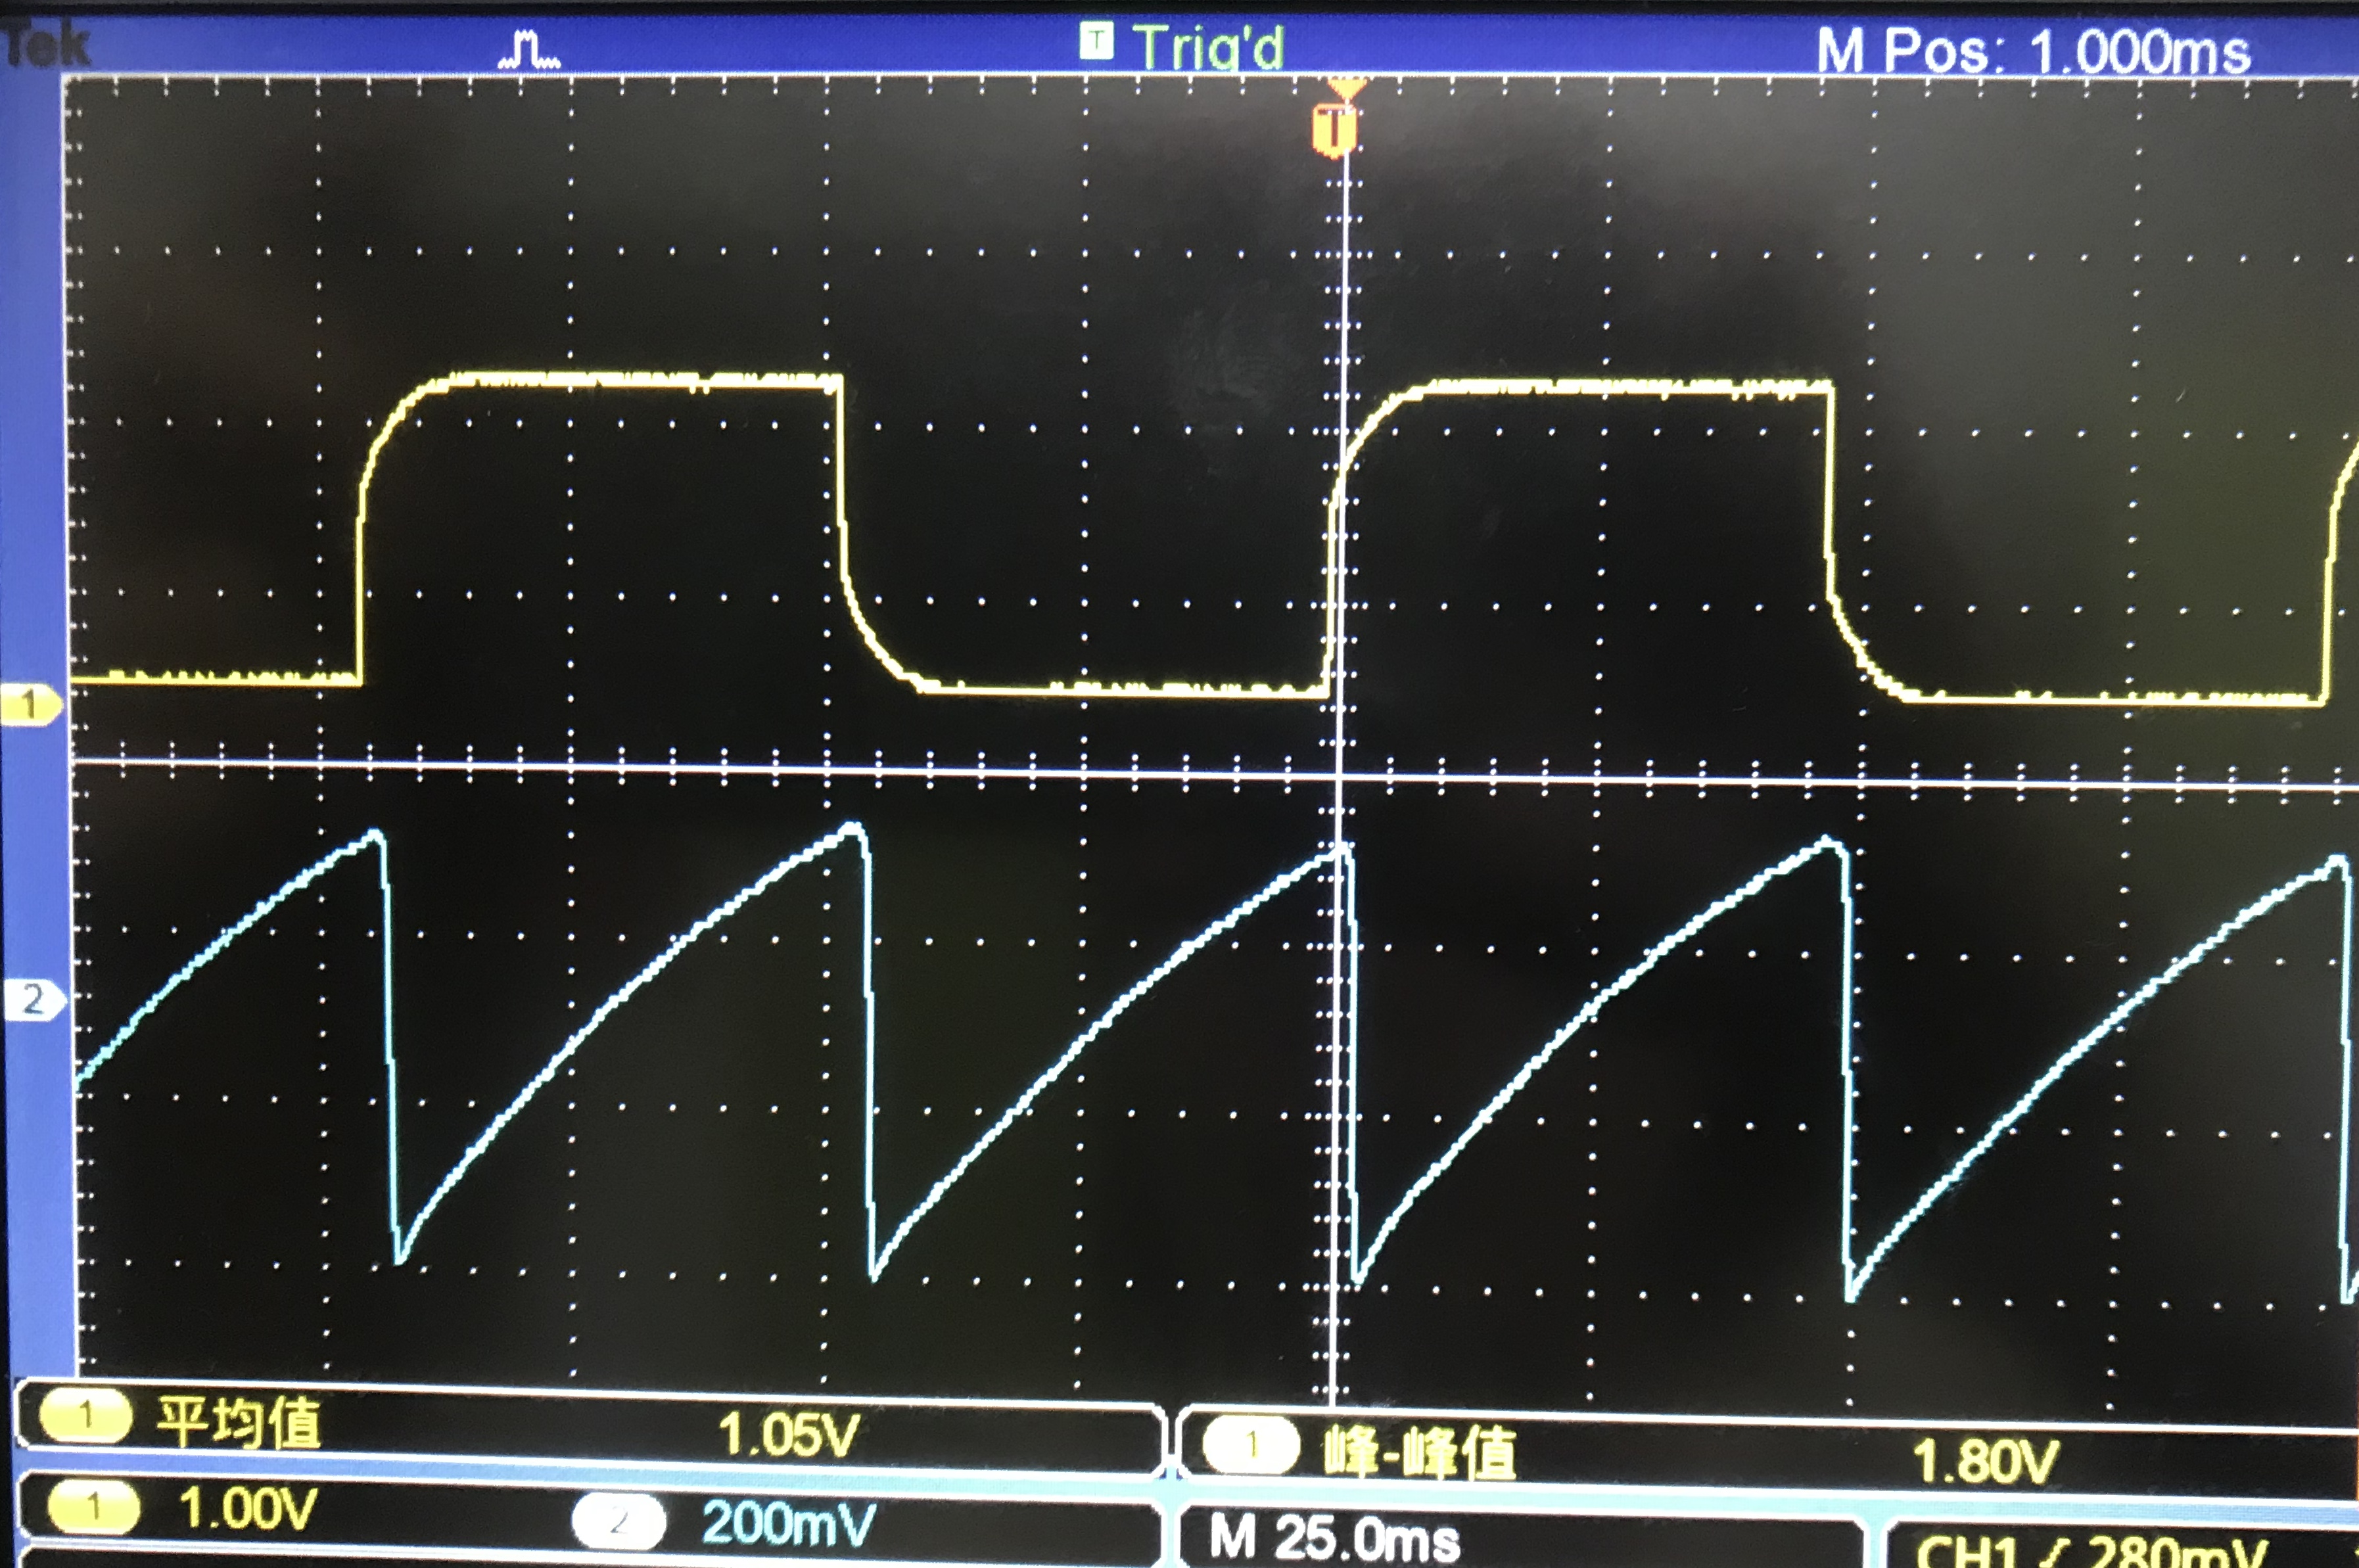
\includegraphics[width=4.3cm]{22}
}
\subfigure[扫场上沿恰为总磁场为0]{
\label{fig:subfig:c}
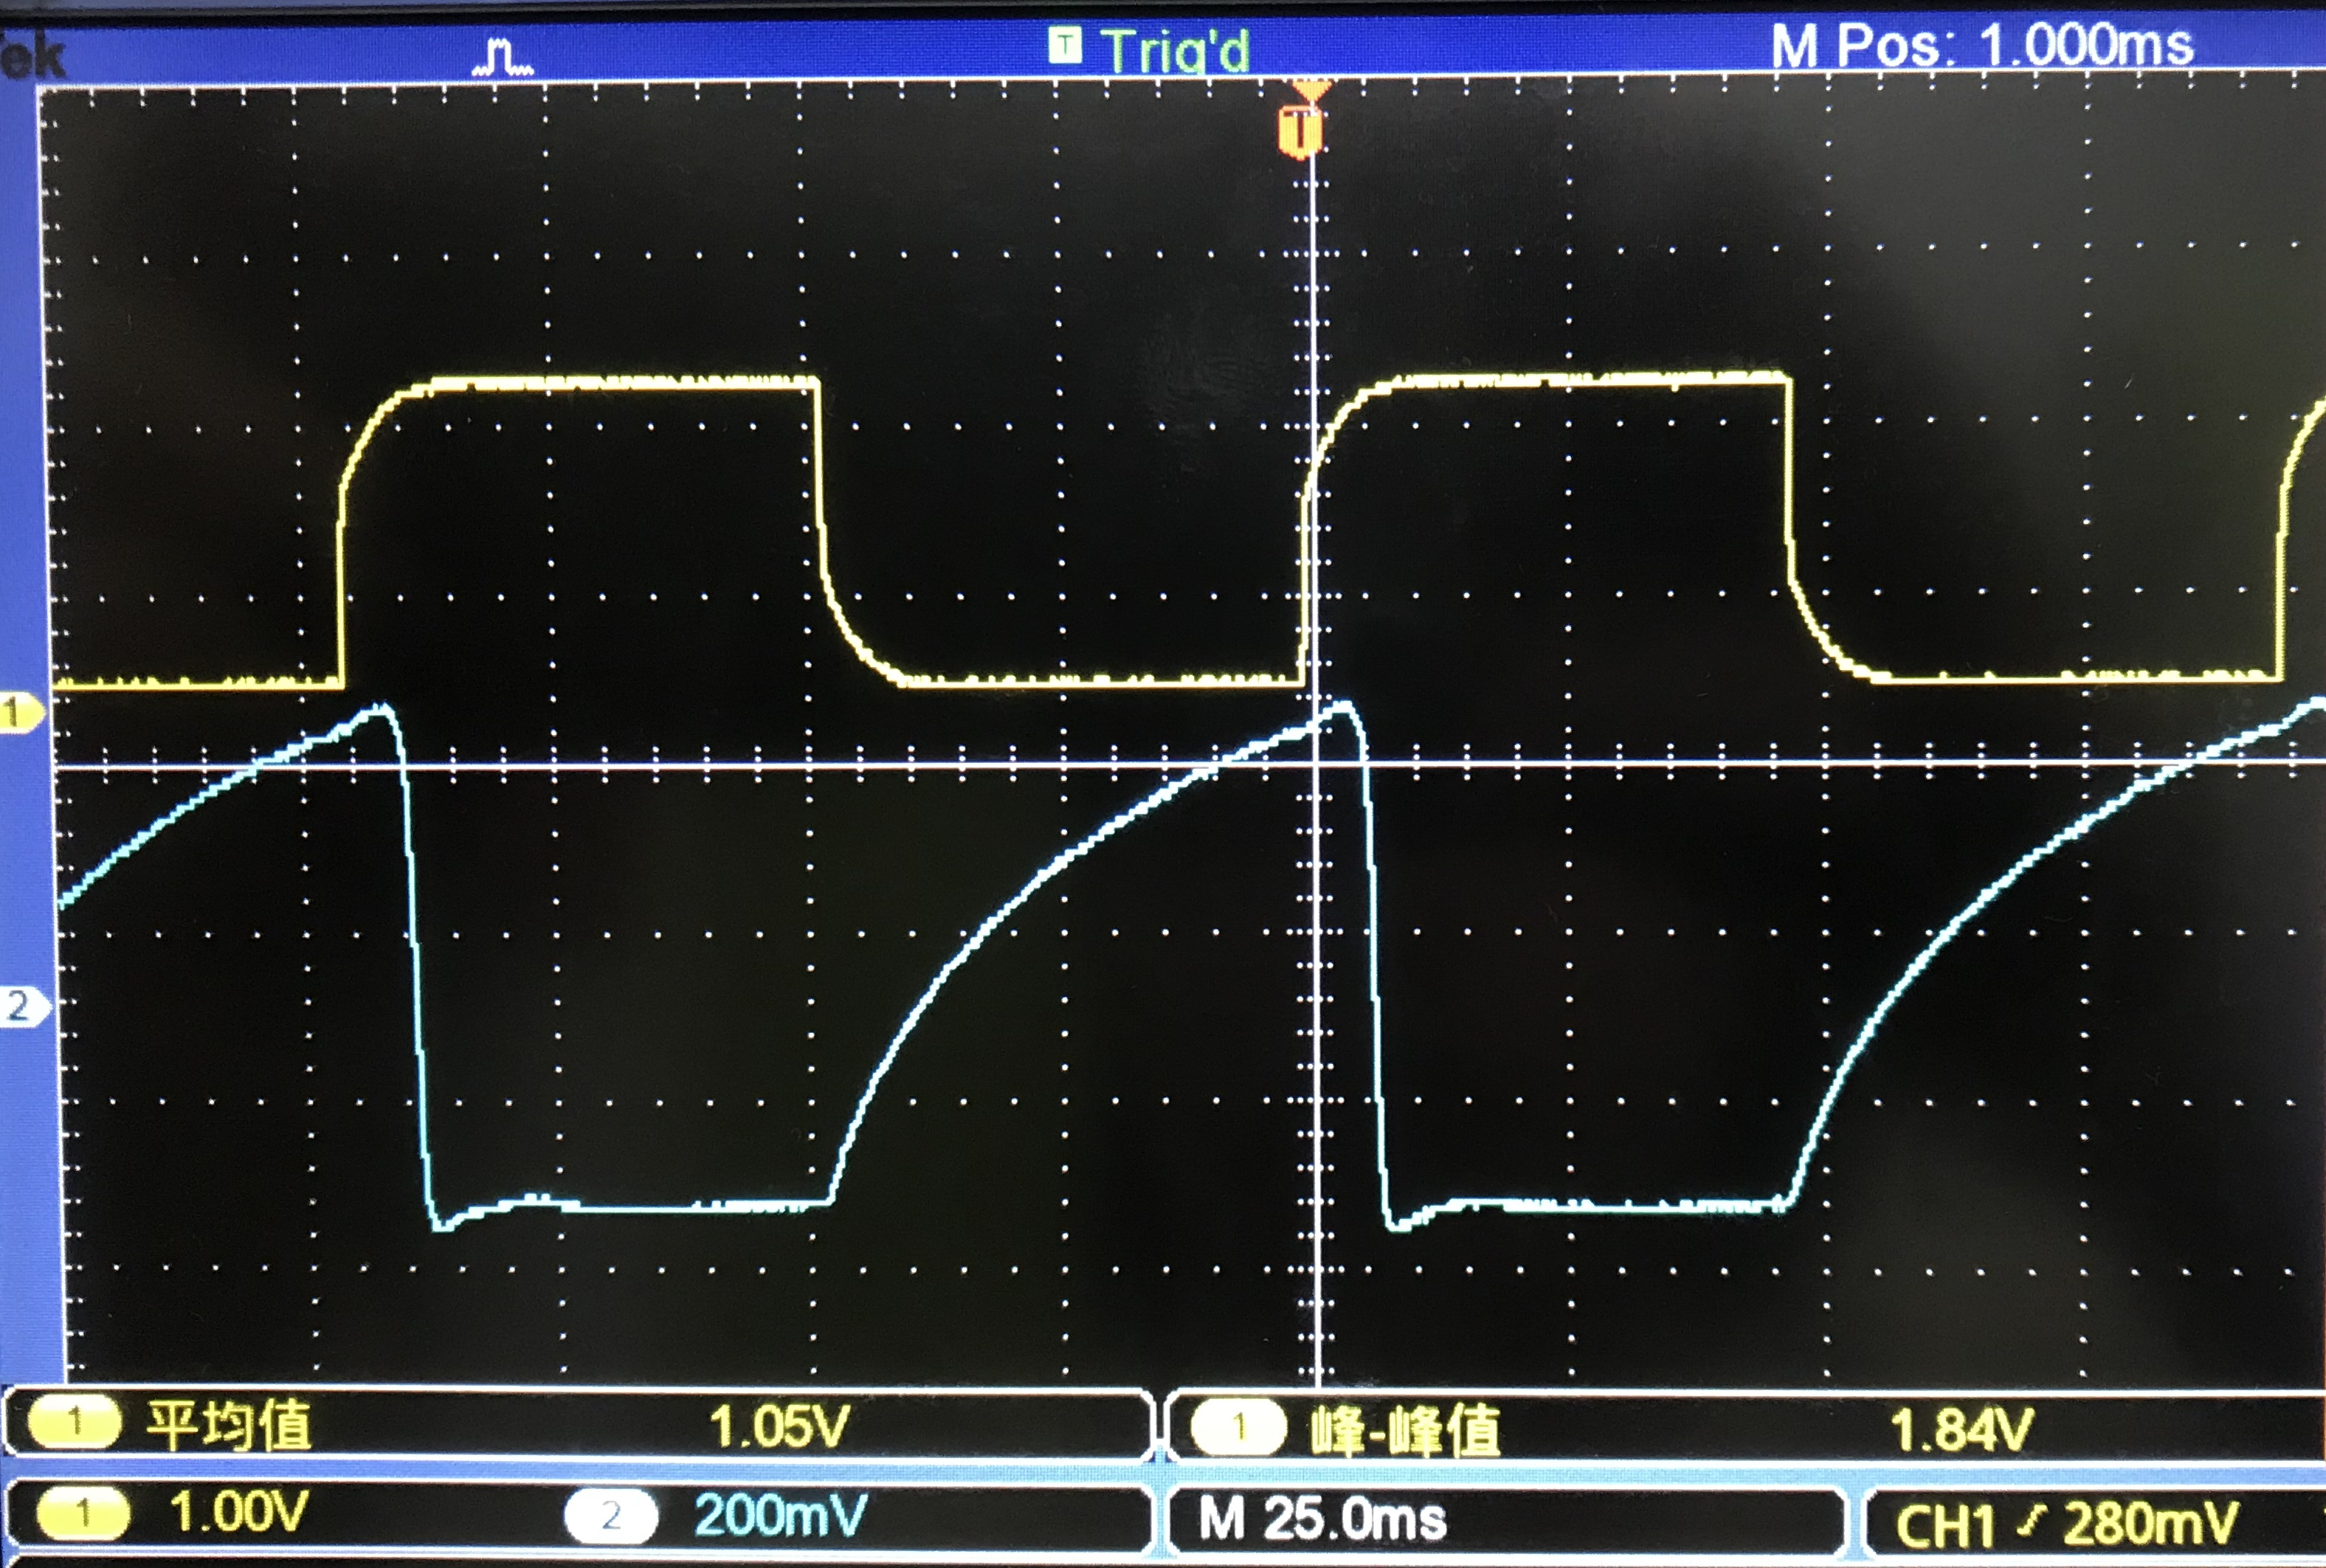
\includegraphics[width=4.3cm]{23}
}
\end{figure}
外加磁场前,基态中各塞曼子能级上的粒子数接近热平衡,对光的吸收能力最强;增大水平场后发生光抽运,粒子逐渐被抽运倒$M_F=+2$子能级上,能吸收的光粒子数减少,透过的光增加,观察到示波器上光信号逐渐增强;故当扫场磁场在过0时得到如上信号。

\noindent\textbf{2.测量磁共振信号}
\newline 测得垂直场电流$I=0.63A$,其余数据如下
\begin{table}[H]
\centering
\begin{tabular}{|c|c|l|l|l|l|l|}
\hline
\multirow{2}{*}{扫场} & \multirow{2}{*}{水平场} & \multirow{2}{*}{}                                                          & \multicolumn{2}{c|}{87Rb}  & \multicolumn{2}{c|}{85Rb}  \\ \cline{4-7} 
                    &                      &                                                                            & 1            & 2           & 1            & 2           \\ \hline
\multirow{3}{*}{正}  & \multirow{3}{*}{正}   & 水平场电流/A                                                                    & 0.1          & 0.139       & 0.204        & 0.242       \\ \cline{3-7} 
                    &                      & 对应磁场/GS                                                                    & 0.469        & 0.652       & 0.957        & 1.136       \\ \cline{3-7} 
                    &                      & $B_{\mbox{水平1}}$(GS) & \multicolumn{2}{c|}{0.561} & \multicolumn{2}{c|}{1.047} \\ \hline
\multirow{3}{*}{正}  & \multirow{3}{*}{反}   & 水平场电流/A                                                                    & 0.277        & 0.316       & 0.381        & 0.421       \\ \cline{3-7} 
                    &                      & 对应磁场/GS                                                                    & 1.300        & 1.483       & 1.788        & 1.976       \\ \cline{3-7} 
                    &                      & $B_{\mbox{水平2}}$(GS) & \multicolumn{2}{c|}{1.391} & \multicolumn{2}{c|}{1.882} \\ \hline
\multirow{3}{*}{反}  & \multirow{3}{*}{反}   & 水平场电流/A                                                                    & 0.205        & 0.24        & 0.31         & 0.346       \\ \cline{3-7} 
                    &                      & 对应磁场/GS                                                                    & 0.962        & 1.126       & 1.455        & 1.624       \\ \cline{3-7} 
                    &                      & $B_{\mbox{水平3}}$(GS) & \multicolumn{2}{c|}{1.044} & \multicolumn{2}{c|}{1.539} \\ \hline
\end{tabular}
\end{table}
故计算得,\textbf{(1)对$^{87}Rb$}

$B_{\mbox{共}}=\frac{1}{2}(B_{\mbox{水平1}}+B_{\mbox{水平2}})=0.976GS$,

对应$g_F=0.476$,误差4.8\%。

$B_{\mbox{地水平}}=\frac{1}{2}(B_{\mbox{水平3}}-B_{\mbox{水平1}})=0.242GS$。

\textbf{(2)对$^{85}Rb$}

$B_{\mbox{共}}=\frac{1}{2}(B_{\mbox{水平1}}+B_{\mbox{水平2}})=1.464GS$,

对应$g_F=0.317$,误差4.8\%。

$B_{\mbox{地水平}}=\frac{1}{2}(B_{\mbox{水平3}}-B_{\mbox{水平1}})=0.246GS$。

\textbf{(3)地磁场}

故$B_{\mbox{地水平}}=0.244GS$;

$B_{\mbox{地垂直}}=0.370GS$;

地磁场大小为$B_{\mbox{地}}=\sqrt{B_{\mbox{地水平}}^{2}+B_{\mbox{地垂直}}^{2}}=0.443GS$

\section{误差分析}
由于信号不稳定,而且是由人眼判断达到临界值,因此导致度数不准确,引起了一定的误差。

\section{结论}
电子吸收圆偏振光后能发生光抽运现象,可以用扫场的方法来观察到该现象;在另加线偏振射频场的情况下,塞曼子能级间发生磁共振,也可以用扫场的方法观察;根据磁共振时测得的水平场可以计算得原子的$g_F$因子和地磁场大小。

\section{参考文献}
\small
\noindent[1]北师大物理实验教学中心,近代物理实验2讲义p63-72,2019.
\begin{figure}[H]
\centering
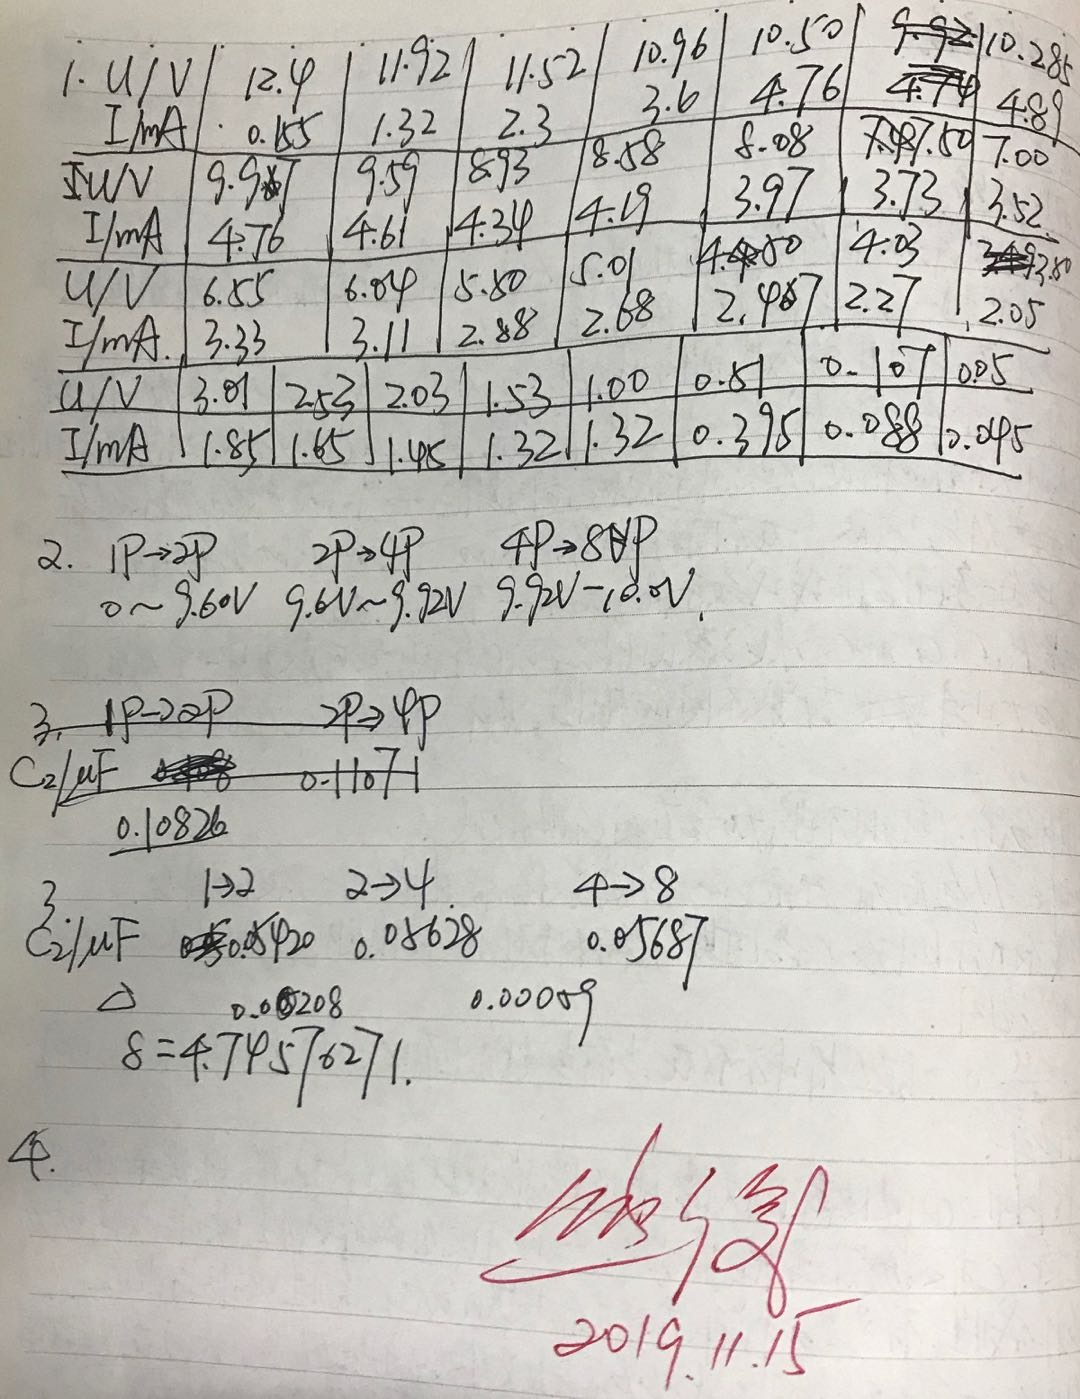
\includegraphics[width=14cm]{record}
\end{figure}

\end{document}